\section*{Reliable set of sled's angle}
    Considering that the rope remains continuously under tension while the robot is moving, then the evolution of the angle $x_4$ of the sled relative to the towing vehicle is described by the \textit{Differential Equation}~\ref{eq:phi}.

    We are able to find the trajectory of the sled by computing the interval containing the angle $x_4$, considering that initially $x_4$ belongs to $[-\pi/2; \pi/2]$. Then by applying the \textit{Differential Equation}~\ref{eq:phi} on this interval, knowing the control vector $u$, we end up obtaining a fine interval framing the real angle $x_4$, independently of the initial angle as we can see on the \textsc{Figure}~\ref{fig:integration}.

    \begin{figure}[!htb]
        \centering
        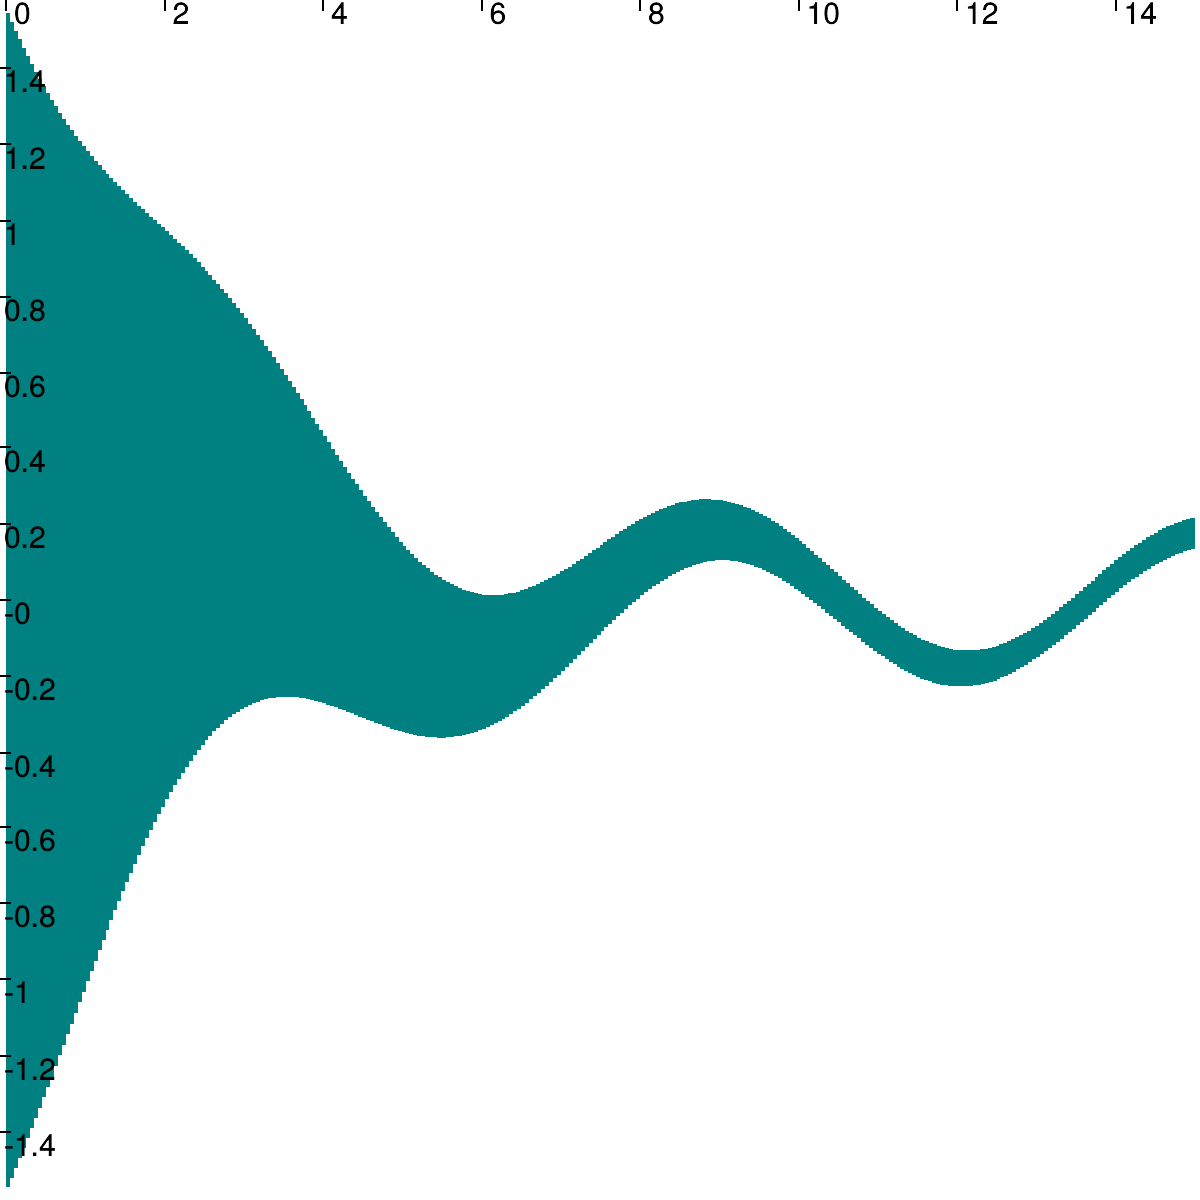
\includegraphics[width=0.35\textwidth]{imgs/integration_example.png}
        \caption{\label{fig:integration} Integration example using intervals}
    \end{figure}